\chapter{拐点暴涨模型在超引力中的实现}%
\label{chap:inflection_model}
电磁相互作用、弱相互作用、强相互作用在粒子物理的标准模型中得到了整合,然而主流
观点认为标准模型与广义相对论无法兼容。另外标准模型也无法解释暗物质与暗能量、中微子
质量、物质与反物质不对称等现象,因此需要拓展标准模型。由于Coleman-Mandula定理
的存在,只有通过放松条件,允许包含反对易算符才能引入超对称性,使得拉格朗日
作用量在玻色场和费米场之间的变换下保持不变。引入超对称性后得到的场论称为超对称
理论。$\mathcal{N}=1$时,超对称算符只有一个,称为简单超对称理论。$\mathcal{N}>1$时
,称为拓展超对称理论。

超对称理论引入的对称性可以\textbf{整体}的,也可以是\textbf{局域}的。
我们提到的\textbf{超引力}理论正是超对称理论的一种局域版本,因为当引入的是局域
的超对称性时,超对称模型能够自然地将引力相互作用包含进来。

超引力作为一种可能地统一描述四种基本相互作用的理论,将其作为理论框架,从中构造
有效的暴涨模型,我们认为是合理的。

这一章论述在$\mathcal{N}=1$的超引力中利用平移对称性构造跑动动能暴涨模型,并以此为出发点对场进行
正则归一化,从而得到符合拐点暴涨模型的势函数。
% 超引力中的暴涨模型简介
\section{暴涨在超引力中的实现}
在超引力中嵌入暴涨模型的研究已经超过三十年了,第一个在超引力中实现的暴涨模型——
混沌暴涨可追溯之1983年
\citep{goncharov1984chaotic},与混沌暴涨的一般化模型的提出仅相隔几个月。 

基于超引力构建的大多数旧暴涨模型\citep{freedman1989progress,deser1976consistent,wess1992supersymmetry}都遇到了$\eta$问题\citep{yamaguchi2011supergravity}:
由于F项势中包含$e$指数因子$e^{{\lvert
\Phi\rvert}^2}$,这一因子使得标量场获得一个与哈勃参数同量级的质量项,
这就使得慢滚参数之一的$\eta$变得大于一,从而破坏了慢滚条件,标量场将迅速
滚到暴涨势的极小值处而不能形成合理的暴涨过程。
如果是小场暴涨模型的话,还可以通过调节参数使得暴涨势在某个区间变得较为平坦,从而
使暴涨过程顺利发生。但对于大场暴涨模型而言,调节参数的方法几乎不可行。最简单的
解决$\eta$问题的方法是将平移对称性(shift symmetry)引入K\"ahler势中\citep{kawasaki2000natural,kawasaki2001natural}。
不过直接引入平移对称性,会导致暴涨势不存在下确界的问题\citep{kawasaki2000natural,kawasaki2001natural}。

除了通过调节参数的方法以外\citep{linde2015single,roest2015cosmological,goncharov1984chaotic},有两种一般性的方法可以解决暴涨势无下确界的问题。
第一种方法是引入额外的稳定场$S$\citep{kawasaki2000natural,kawasaki2001natural,kallosh2010new,kallosh2011general}。第二种方法是将满足平移对称性的暴涨场的4次方项
引入K\"ahler势中\citep{ketov2016single,ketov2014inflation,izawa2007supersymmetric,ketov2014generic}。

早期有一类双场理论
\citep{kallosh2010new},$S=s
e^{i\theta}/\sqrt{2}$和$\Phi=(\phi+i\chi)/\sqrt{2}$,以及超势$W=Sf(\Phi)$,其中$f(\Phi)$是实全纯函数,满足$\bar{f}(\Phi)=f(\Phi)$。
模型中有两个超场,或者四个实标量场,$s$,$\theta$,$\phi$和$\chi$,其中只有
一个实场对应暴涨场,参与宇宙学演化。通常选取$\phi$或$\chi$作为暴涨场,$S$作为辅助场。
K\"ahler势的函数形式可以取做$K=K({(\Phi-\bar{\Phi})}^2,S\bar{S})$。这种情形下,暴涨势$V$在$s=\chi=0$处有极值,如果该极值同时也
是全局最小值,那么标量场$\phi$将扮演正则归一化的暴涨场,暴涨势为$V(\phi)=|f(\phi/\sqrt{2})|^2$,且暴涨过程发生在$s=\chi=0$的方向上。为了与宇宙学观测保持一致,
暴涨模型需要给出符合观测的宇宙学参数$n_{s}$和$r$,这一点总是可以通过选取合适
的函数$f(\Phi)$来做到。

% 跑动动能项暴涨模型
\section{跑动动能项暴胀模型}
其次是\textbf{跑动动能项暴胀}模型,是指场的质量在暴胀期间会随场的变化而变的模型
。对于慢滚暴胀模型,习惯假设暴胀场是弱耦合场,其拉氏量中的动能项在暴胀期间及暴
胀结束后不会发生大的改变。又为了暴胀能够产生,通常利用对称性产生平坦的势能。如
果不利用对称性,通常需要精细调节参数来获得平坦的势能,且需要挑选能够使暴胀发生
的初始位置。后来,有人提出了一类新的暴胀模型,丢弃了动能项的变化被忽略的假设。
在整个暴胀期间,动能项的变化不能被忽略,在某些情况下,这种变化甚至能明显地影响
到暴胀场的动力学。这样的模型被称为\textbf{跑动动能暴胀}模型。

假设实标量场$\phi$有如下形式的拉氏量,
\begin{equation}
  \mathcal{L} =
  \frac{1}{2}f(\phi)\partial^{\mu}\phi\partial_{\mu}\phi-V(\phi),
\end{equation}
假设场$\phi$在某个区间时,$f(\phi)$的行为能够近似为$f(\phi)\approx
\phi^{2n-2}$,$n$为给定的整数。则对场$\phi$作正则归一化之后,$\hat{\phi}\equiv
\phi^{n}/n$,势能函数将会变得更加平坦。例如,当$n=2$时,二次(四次)方势能函数,$V(\phi)\propto
\phi^2(\phi^{4})$,将变成线性(二次)势能$V(\hat{\phi})\propto
\hat{\phi}(\hat{\phi}^2)$。因此暴胀场的动力学非常依赖其动能项。

再举一个例子,
\begin{equation}
  f(\phi) = \kappa + \phi^2. 
\end{equation}
其中$0 < \kappa \ll 1$。因此当$\phi \gtrsim \sqrt{\kappa}$时,$f(\phi)
\approx \phi^2$。当$\phi \ll \sqrt{\kappa}$时,$f(\phi)\approx
\sqrt{\kappa}$。因此,标量场$\phi$将按如下方式进行正则归一化
\begin{equation}
  \hat{\phi} = 
  \begin{cases}
    \frac{\phi^2}{2}, \qquad & \phi \gg \sqrt{\kappa} \\
    \sqrt{\kappa},\qquad & \phi \ll \sqrt{\kappa}
  \end{cases}
\end{equation}
故而当$V(\phi)=m^2\phi^2/ 2$时,正则场的势能函数为
\begin{equation}
  V(\hat{\phi}) \simeq 
  \begin{cases}
    m^2\hat{\phi},\qquad & \hat{\phi} \gg \kappa \\
    \frac{m^2}{2\kappa} \hat{\phi}^2,\qquad & \hat{\phi} \ll \kappa
  \end{cases}
\end{equation}
从这个例子可以发现,从一个形式简单的拉氏量出发,经过正则归一化,能够轻松实现势能
函数从线性形式到二次函数的转变。
原则上,我们可以把正则场$\hat{\phi}$满足的拉氏量作为出发点,得到的暴胀模型拥有
相同的动力学。然而,这种方式难以从理论上解释为何暴胀场的势能取这样一种特定的函数
形式。



% 构造拐点暴涨模型
\section{构造拐点暴胀模型}
如3.1节中提到的解决$\eta$问题\citep{stewart1995inflation,linde1994hybrid,linde1997hybrid,panagiotakopoulos1997hybrid}除了通过调节参数以外,一般有两类方法。
其中一种是将平移对称性引入K\"ahler势中$K(\phi-\phi^\dagger)$,这样暴胀场不会出现在K\"ahler势中,消失的指数因子保证了势能的平坦性。这种情形下,能够得到幂指数势能$V(\phi)\propto
\phi^n$的混沌暴胀。

有作者\citep{takahashi2010linear,nakayama2010running,kasuya2014flat}将手征场$\phi$的类Nambu-Goldstone平移对称性推广到了一般形式$\phi^n\rightarrow
\phi^n+C$,使得K\"ahler势是$\left(\phi^n-\phi^\dagger\right)$的函数。
为了获得合理的势能形式,应当在K\"{a}hler势和超势中分别加入一个小的shift对称性破缺项$\kappa|\phi|^2$和$\lambda\phi^m
X$,此处有$\kappa,\lambda\ll
1$以及外场$X$。这样可以获得幂指数为分数的标量势能$V(\phi)\propto
\phi^{m/n}$,标量谱指标$n_s$以及张标比$r$近似为
$n_s=1-(1+\frac{m}{n})\frac{1}{N}$和$\frac{8m}{n}\frac{1}{N}$\citep{nakayama2010running}。
由于模型中动能项的系数是场依赖的:$(\kappa+n^2|\phi|^{2n-2})\partial_{\mu}\phi\partial^{\mu}\phi^{\dag}$,这就是所谓的跑动动能项暴胀。


在\citep{gao2015inflection}中,作者用单手征超场构造出了一个拐点暴胀模型,与Planck
2015年的结果相一致。在暴胀结束后,该模型进入一个非超对称德-西特真空,能够用于解释宇宙近期的加速膨胀。
在最小超对称标准模型的框架下,通过规范不变的平坦方向\textit{udd}或\textit{LLe}首次构造出了拐点暴胀模型\citep{allahverdi2006gauge},并得到了发展\citep{allahverdi2007term,enqvist2010inflection,hotchkiss2012observable,chatterjee2015bound}。


\subsection{带跑动动能项的多项式超势}
对于慢滚暴胀模型,习惯假设暴胀场是弱耦合场,其拉氏量中的动能项在暴胀期间及暴胀
结束后不会发生大的改变。又为了暴胀能够产生,通常利用对称性产生平坦的势能。如果
不利用对称性,通常需要精细调节参数来获得平坦的势能,且需要挑选能够使暴胀发生的
初始位置。后来,有人提出了一类新的暴胀模型,丢弃了动能项的变化被忽略的假设。在
整个暴胀期间,动能项的变化不能被忽略,在某些情况下,这种变化甚至能明显地影响到
暴胀场的动力学。这养的模型被称为\textbf{跑动动能暴胀}模型。


K\"ahler势在手征超场$\phi$的广义平移对称性变换下保持不变:
\begin{equation}
    \phi^n \rightarrow \phi^n + C,
\end{equation}

因此,它必然是$i\chi \equiv (\phi^n - \phi^{n\dagger})$的函数:
\begin{equation}
    K = \sum_{l=1}\frac{c_l}{l}{\left(\phi^n-\phi^{n\dagger}\right)}^l
    =
    i c_1(\phi^n-\phi^{n\dagger})-\frac{1}{2}{\left(\phi^n-\phi^{n\dagger}\right)}^2+\cdots.
\end{equation}

系数$c_l$是与$1$同量级的常数。在暴胀期间,$\chi$一直稳定在极小值处,所以$l\ge
3$的项对动能的贡献可以忽略\citep{takahashi2010linear}。对$l\le2$的项,$\chi$稳定在$\chi_{\text{min}}\simeq
c_1$。

为了使暴胀模型可行,需要在K\"ahler势中添加一个微小的平移对称性破缺项:
\begin{equation}
    \Delta{K} = \kappa \left|\phi\right|^2,
\end{equation}
系数满足条件$0< \kappa \ll 1$。

与\citep{nakayama2010running}不同,我们假设超势满足一个更一般的形式\citep{nakayama2013polynomial,kawasaki2000natural,kawasaki2001natural,kallosh2010new,kallosh2011general}
\begin{equation}
    W = X\left(\sum_{m=0}\lambda_m\phi^m\right)+W_0.
\end{equation}
这里$\lambda_m\ll
1$,$X$是一个额外的手征超场,并且稳定在$X=0$。$\left|W_0\right|\simeq
m_{3/2}$且$m_{3/2}$为引力微子的质量。按照通常的假设,在暴胀过程中$m_{3/2}$远远小于哈勃参数,所以在讨论暴胀动力学的时候可以被丢弃。

所以最终的K\"ahler势为
\begin{equation}
    K = \kappa |\phi|^2 + c_1(\phi^n-\phi^{n\dagger}) -
    \frac{1}{2}{(\phi^n-\phi^{n\dagger})}^2 + |X|^2\cdots.
\end{equation}

超势$W$和K\"ahler势共同决定了标量场$\phi$的有效拉式量
\begin{equation}
\begin{split}\label{eq:lagrangian-with-running-kinetic-term}
L &= -K^{\phi\phi^\dagger} \partial_\mu\phi\partial^\mu\phi^\dagger
- V \\
  & = (\kappa + n^2|\phi|^{(2n-2)})
  \partial_\mu \phi \partial^\mu \phi^\dagger - V,
\end{split}
\end{equation}
暴胀场$\phi$的标量势能为
\begin{equation}
\begin{split}
V &= e^K \left[
    D_\phi W{(K^{-1})}^{\phi\phi^\dagger}{(D_\phi W)}^{\star} - 3|W|^2 
    \right]\\
  &=
  e^{\kappa|\phi|^2+c_1(\phi^n-\phi^{n\dagger})-\frac{1}{2}{(\phi^n-\phi^{n\dagger})}^2}{(\sum_m
  \lambda_m|\phi|^m)}^2,
\end{split}
\end{equation}
其中
\begin{equation}
    D_\phi W = \partial_\phi W + (\partial_\phi K) W,
\end{equation}
以及
\begin{equation}
    K^{\phi\phi^\dagger} = \frac{\partial^2 K}{\partial\phi
    \partial\phi^\dagger}
\end{equation}

当${(\kappa/n^2)}^{1/(2n-2)}\ll |\phi| \ll
\kappa^{-1/2}$时,$\kappa$项可以忽略,所以若定义$\hat{\phi} \equiv
\phi^n$,则意味着$\hat{\phi}$在类Nambu-Goldstone平移变换下不变,拉式量
(\ref{eq:lagrangian-with-running-kinetic-term})近似为
\begin{equation}
\begin{split}
    L &= \partial_\mu \hat{\phi}\partial^\mu \hat{\phi}^\dagger -
    e^{-\frac{|c_1|^2}{2}}{(\sum_m \lambda_m|\hat{\phi}|^{m/n})}^2 \\
    &= \partial_\mu \hat{\phi} \partial^\mu \hat{\phi}^\dagger - 
    {(\sum_m \hat{\lambda_m}|\hat{\phi}|^{m/n})}^2,
\end{split}
\end{equation}
其中$i\chi \equiv (\phi^n - \phi^{n\dagger})=i c_1$,$\hat{\lambda}_m\equiv
e^{-\frac{|c_1|^2}{4}}\lambda_m$。

由于平移对称性,$\hat{\phi}$的实部不会出现在K\"ahler势中,所以势能在实方向上相当地平坦使得其成为暴胀场候选者。
虚部获得了比哈勃能标更重地质量,并且在暴胀过程中稳定在极小值处。因此,设$\hat{\phi}\equiv
(\varphi+i \chi)/\sqrt{2}=\varphi/\sqrt{2}+i
c_1/ \sqrt{2}$并得到$\varphi$地标量势能
\begin{equation}\label{eq:varphi_scalar_potential}
    V = {\left[\sum_{m=0}\hat{\lambda}_m
    {\left(\frac{\varphi}{\sqrt{2}}\right)}^{\frac{m}{n}}\right]}^2.
\end{equation}

\subsection{暴胀场的拐点势能}
为了创建一个拐点暴胀模型,我们采用如下形式的超势
\begin{equation}\label{eq:superpotential}
    W = X(\lambda_p\phi^p + \lambda_q e^{i\theta}\phi^q),
\end{equation}
其中幂指数$q > p \le
1$且为整数,系数$\lambda_p$、$\lambda_q$为正实数且不失一般性,$\theta$为第二项的相位。

将 (\ref{eq:superpotential})代入势能函数
(\ref{eq:varphi_scalar_potential})得到
\begin{equation}
  \label{eq:scalar_potential}
\begin{split}
    V &= {\left[ \hat{\lambda}_p {\left(\frac{\varphi}{\sqrt{2}}\right)}^{\frac{p}{n}}
    + \hat{\lambda}_q e^{i\theta}{\left(\frac{\varphi}{\sqrt{2}}\right)}^{\frac{q}{n}}\right]}^2 \\
    &= \hat{\lambda}_p^2 {\left(\frac{\varphi}{\sqrt{2}}\right)}^{\frac{2p}{n}}
    \left[1 + 2\xi\cos\theta {\left(\frac{\varphi}{\sqrt{2}}\right)}^{\frac{q-p}{n}}
    + \xi^2 {\left(\frac{\varphi}{\sqrt{2}}\right)}^{\frac{2(q-p)}{n}}\right],
\end{split}
\end{equation}
其中$\hat{\lambda}_{p,q}\equiv
e^{-\frac{|c_1|^2}{4}}\lambda_{p,q}$和$\xi=|\hat{\lambda}_q/\hat{\lambda}_p|=|\lambda_q/\lambda_p|$。图$(\ref{fig:potential-for-single-inflection-point-inflation})$根据参数$\theta$的变化展示了三种可能的势能曲线。

\begin{figure*}
  \centering
  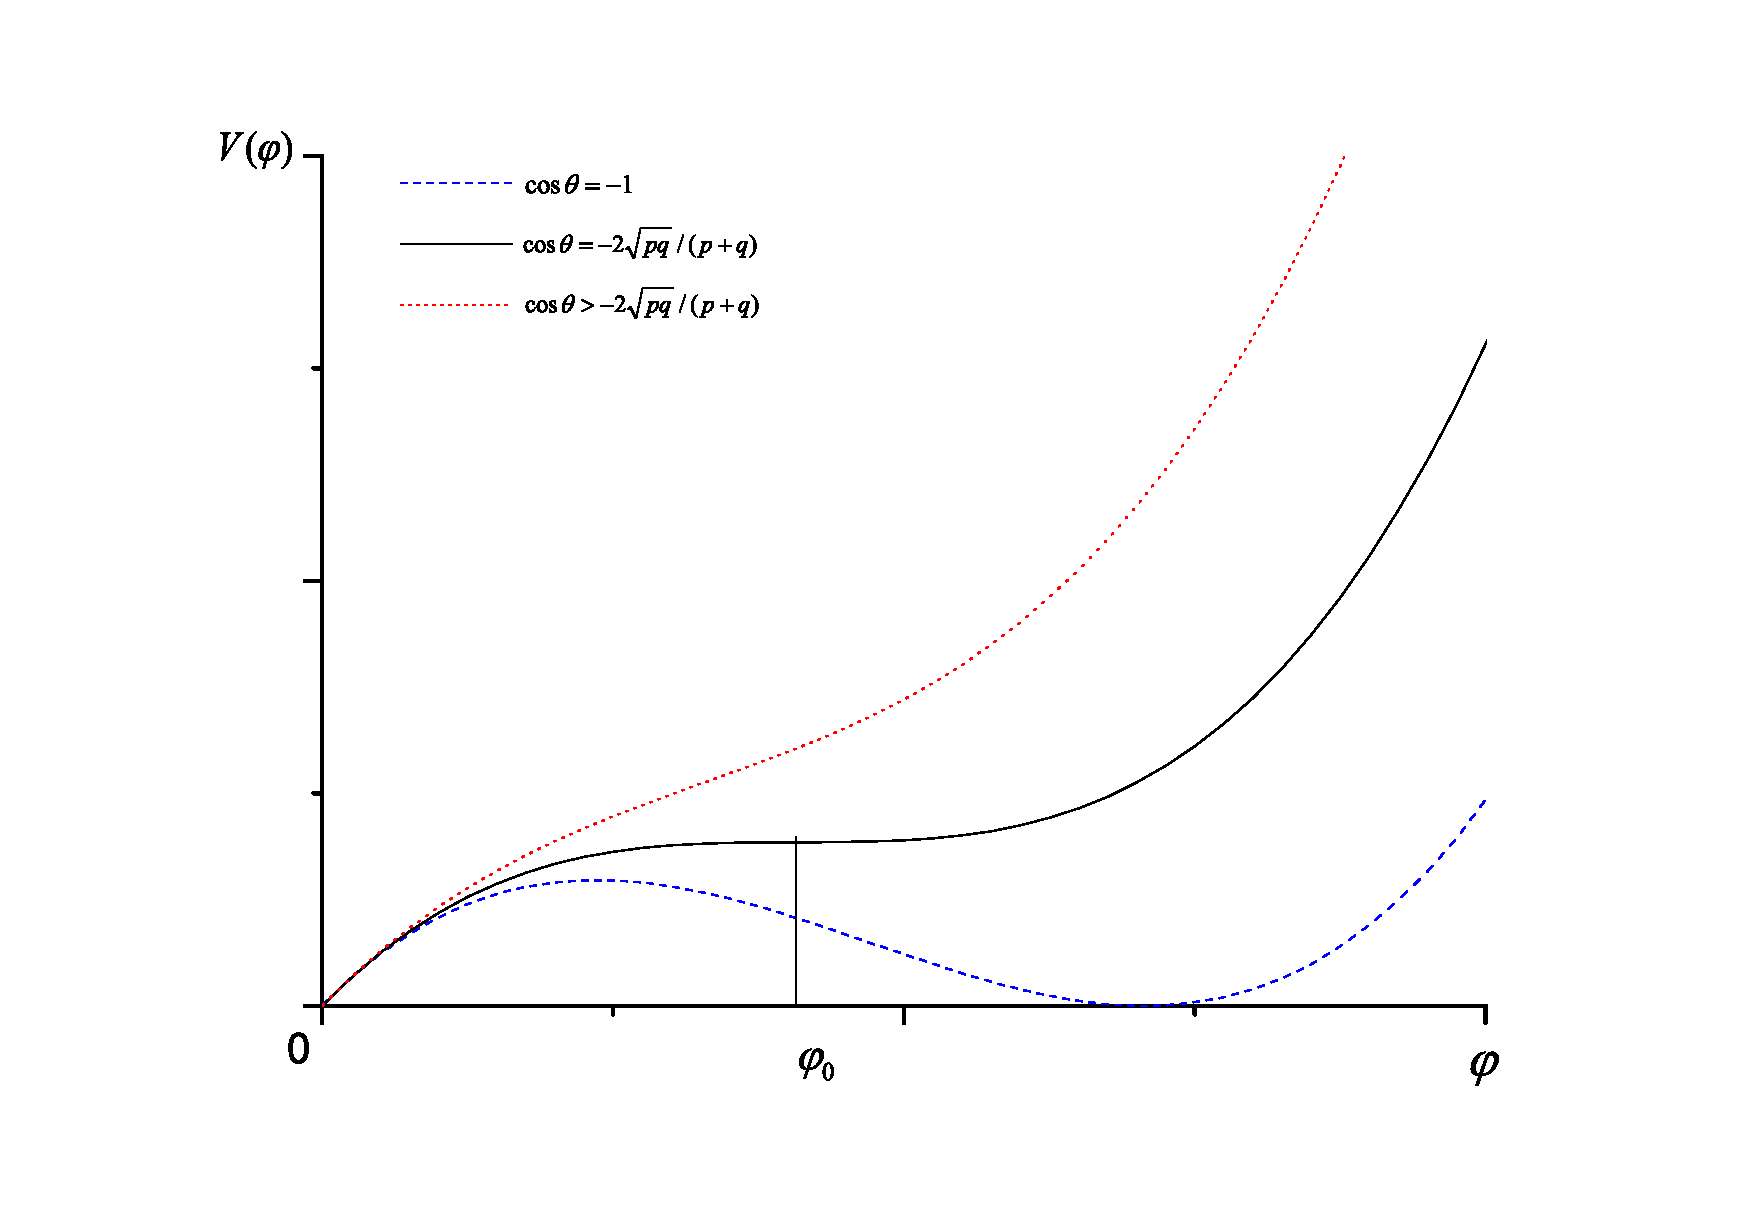
\includegraphics[width=5in]{Img/Graph1.eps}
  \caption{暴胀势能$V(\varphi)$,虚线、实线、点线分别对应$\cos\theta=-1$、$\cos=-2\sqrt{pq}/(p+q)$、$\cos>-2\sqrt{pq}/(p+q)$}\label{fig:potential-for-single-inflection-point-inflation}
\end{figure*}

我们发现当$\cos\theta =
-1$时,势能存在$\varphi=\sqrt{2}{\left(\frac{p}{\xi
q}\right)}^{\frac{n}{q-p}}$和$\varphi=0$处分别存在一个极小值,如图$(\ref{fig:potential-for-single-inflection-point-inflation})$中蓝色虚线所示。当$\cos\theta$逐渐变大,$\varphi=\sqrt{2}{\left(\frac{p}{\xi
q}\right)}^{\frac{n}{/q-p}}$处的极小值逐渐上移被抬起。如果抬起的不够高,那么暴胀场仍有可能被困在假真空之中。

有趣的情况是当$\theta$满足条件
\begin{equation}
  \label{eq:inflection-point-condition}
  \cos\theta = - \frac{2\sqrt{pq}}{p+q}. 
\end{equation}
局部最大值和右侧极小值在$\varphi_0=\sqrt{2}{\left(\frac{1}{\xi}\sqrt{\frac{p}{q}}\right)}^{\frac{n}{q-p}}$处重合,假真空消失。这个点被称为反射点,此处暴胀势能为
\begin{equation}
  V(\varphi_0) = \hat{\lambda}^2_{p} \left( \frac{p}{q}+\frac{4p}{p+q}+1\right)
  {\left(\frac{p}{\xi^2 q}\right)}^{\frac{p}{q-p}},
\end{equation}
并且势能$V$的一阶、二阶导数在$\varphi_0$处都等于零。值得注意的是反射点的势能表达式中不含$n$,表明给定不同的参数$n$在反射点的势能大小都相同。在反射点的势能大小都相同。
因为$\varphi_0$附近势能非常平坦,因此模型预言的标量谱指标以及张标比都能落在Planck
2015年数据限制的$1\sigma$置信水平的区域中。

当$\cos\theta > -
\frac{2\sqrt{pq}}{p+q}$,则势能不再有平坦的区间,将重现出势能为幂函数的暴胀模型。

另外一件值得注意的事情是当选定参数为某些值的时候,势能在原点附近是一个奇函数,这将导致暴胀场在暴胀结束后产生期待之外的行为。
不过当标量场满足条件
\begin{equation}
  \varphi < \sqrt{2} {\left(\frac{\kappa}{n^2}\right)}^{\frac{n}{2n-2}}.
\end{equation}
时,式$(\ref{eq:lagrangian-with-running-kinetic-term})$中动能项里的$\kappa$将不能忽略。正如前面小节中提到的那样,此时正则归一的动力学变量不再是$\varphi$,而是标量场$\phi$。于是对应的势能也不再是图$(\ref{fig:potential-for-single-inflection-point-inflation})$中所示,而是${\left(\sum_m
\lambda_m \left\lvert \phi \right\rvert^{m}\right)}^2$。
当$\phi$增加时,SUSY破缺质量项$m_{\phi}\left\lvert \phi\right\rvert
^2$将会主导势能变化\citep{nakayama2010running},因此标量场将会在原点附近不断振荡然后重新加热宇宙。

现在开始把注意力集中在拐点暴胀势能上。因为参数$\theta$满足条件$(\ref{eq:inflection-point-condition})$,因此当参数$n$、$p$和$q$给定时,只剩下两个自由参数$\hat{\lambda}_{p}$和$\xi$。
暴胀场的势能$(\ref{eq:scalar_potential})$将变成
\begin{equation}
  \label{eq:inflection-poin-potential}
  V(\varphi) = \hat{\lambda}^2_{p}
  {\left(\frac{\varphi}{\sqrt{2}}\right)}^{\frac{2p}{n}} 
  \left[ 1-4\xi \frac{\sqrt{pq}}{p+q}
  {\left(\frac{\varphi}{\sqrt{2}}\right)}^{\frac{q-p}{n}} + \xi^2 
{\left(\frac{\varphi}{\sqrt{2}}\right)}^{\frac{2(q-p)}{n}}\right].
\end{equation}

\subsection{慢滚近似}
式$(\ref{eq:PSRA_epsilon})$和$(\ref{eq:PSRA_eta})$为势能慢滚参数$\epsilon$和$\eta$的定义。在近似到一阶的情况下,标量功率谱指标$n_{s}$和张标比$r$用慢滚参数表示的表达式为
\begin{align}
  \label{eq:ns-in-slow-roll-parameter}
  & n_{s} \simeq 1 - 6\epsilon + 2\eta, \\
  \label{eq:eta-in-slow-roll-parameter}
  & r \simeq 16\epsilon.
\end{align}
暴胀期间的e-folding数可以用下面的积分式计算
\begin{equation}
  \label{eq:e-folding-number-with-potential-integral}
  N = \int_{\varphi_{f}}^{\varphi_{i}} \frac{V}{V^\prime} d\varphi, 
\end{equation}
$\varphi_{i}$和$\varphi_{f}$分别为暴胀开始和结束的时刻,并且$\varphi_{f}$的值由
$\text{Max} \{\epsilon(\varphi_{f}), \eta(\varphi_{f})\}=1$决定。

参数$\hat{\lambda}_{p}$的限制条件为曲率扰动的振幅
\begin{equation}
  \label{eq:amplitude-of-curvature-perturbation-by-Planck}
  \mathcal{P}_{\mathcal{R}} = \frac{V}{24\pi^2\epsilon}.
\end{equation}
根据 Planck 2015 的数据,$\mathcal{P}_{\mathcal{R}}(k_0)=2.19\times
10^{-9}$。因此给定$n,p,q$的值之后,就能得到$\hat{\lambda}_{p}$和$\xi$的关系。
针对不同的$n$、$p$、$q$的取值,我们计算了$\hat{\lambda}_{p}$和$\xi$的关系并绘制了图$(\ref{fig:Ln-1-2})$、$(\ref{fig:L2-p-4})$和$(\ref{fig:L2-1-q})$。
图$(\ref{fig:LN-50})$针对给定的$n$、$p$、$q$,但是不同的e-folding数$N=60$和$N=50$。

\begin{figure}
  \centering
  \includegraphics[width=5in]{Img/Ln,1,2.eps}
  \caption{e-folding数$N=60$,参数$(p,q)$为$(1,
  2)$,$n=2,3,4$时,为了与Planck数据给出的曲率扰动相一致,参数$\hat{\lambda}$和$\xi$必须满足的关系。}\label{fig:Ln-1-2}
\end{figure}

\begin{figure*}\small
  \centering
  \includegraphics[width=5in]{Img/L2,p,4.eps}
  \caption{e-folding数$N=60$,参数$(n,q)$为$(2,
  4)$,$p=1,2,3$时,为了与Planck数据给出的曲率扰动相一致,参数$\hat{\lambda}$和$\xi$必须满足的关系。}\label{fig:L2-p-4}
\end{figure*}

\begin{figure*}\small
  \centering
  \includegraphics[width=5in]{Img/L2,1,q.eps}
  \caption{e-folding数$N=60$,参数$(n,p)$为$(2,
  1)$,$q=2,3,4$时,为了与Planck数据给出的曲率扰动相一致,参数$\hat{\lambda}$和$\xi$必须满足的关系。}\label{fig:L2-1-q}
\end{figure*}

\begin{figure*}\small
  \centering
  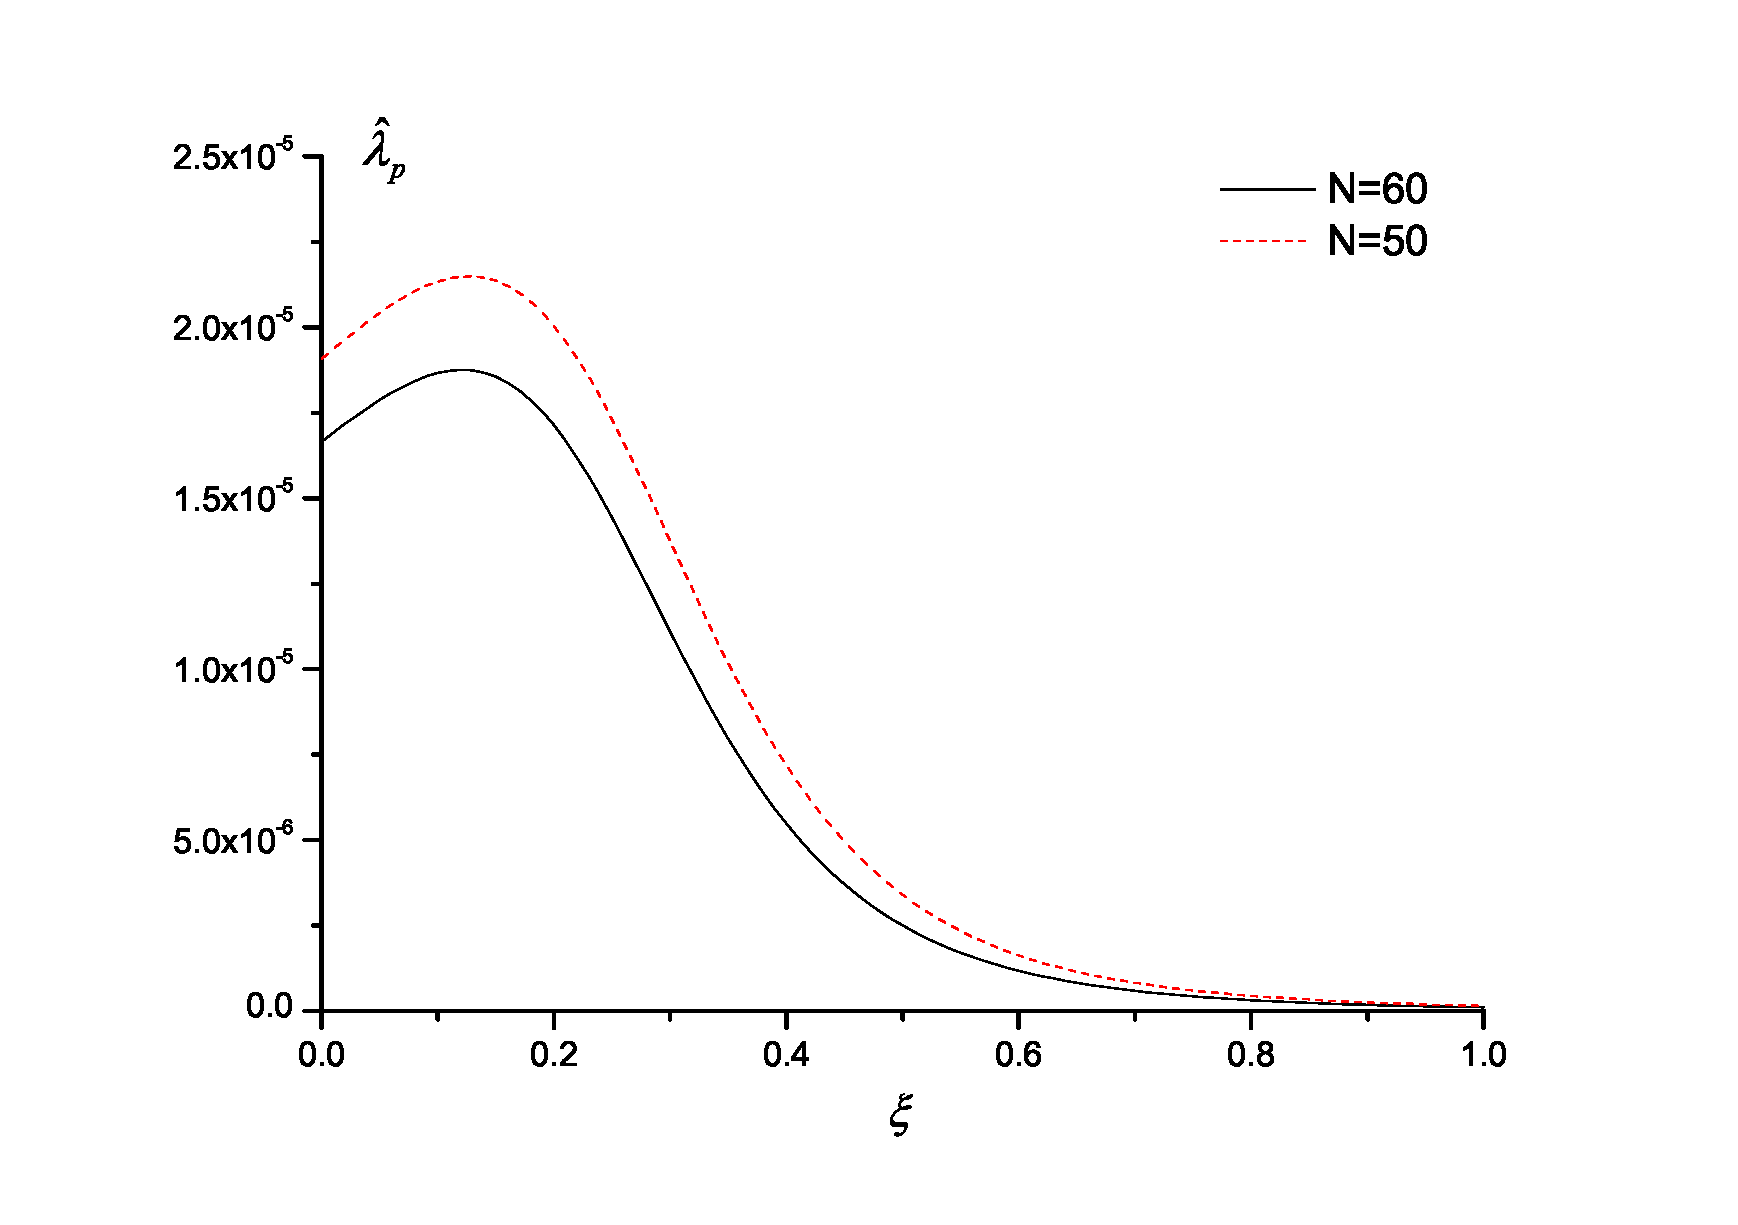
\includegraphics[width=5in]{Img/LN=50.eps}
  \caption{参数$(n,p,q)$为$(2,1,2)$,e-folding数分别为$N=60$和$N=50$时,为了与Plack数据给出的曲率扰动相一致,参数$\hat{\lambda}$和$\xi$必须满足的关系。}\label{fig:LN-50}
\end{figure*}

\begin{figure*}\small
  \centering
  \includegraphics[width=5in]{Img/Gn,1,2.eps}
  \caption{曲线是当e-folding数为$N=60$时,模型给出的$n_{s}-r$关系。等高线分别为$68\%$和$95\%$置信水平上,$n_{s}$和$r$坐落的区域,由Planck
  2015年TT+lowP数据给出,基准尺度为$k_{\star}=0.002\text{Mpc}^{-1}$。其中参数$(p,
q)$为$(1,2)$,幂指数$n$从上到下分别为$1,2,3,4$。曲线上黑点处对应参数$\xi=0$。}\label{fig:Gn-1-2}
\end{figure*}


\begin{figure*}\small
  \centering
  \includegraphics[width=5in]{Img/G2,p,4.eps}
  \caption{曲线是当e-folding数为$N=60$时,模型给出的$n_{s}-r$关系。其中参数$(n,
q)$为$(2,4)$,幂指数$p$从上到下分别为$3,2,1$。曲线上黑点处对应参数$\xi=0$。}\label{fig:G2-p-4}
\end{figure*}

\begin{figure*}\small
  \centering
  \includegraphics[width=5in]{Img/G2,1,q.eps}
  \caption{曲线是当e-folding数为$N=60$时,模型给出的$n_{s}-r$关系。其中参数$(n,
p)$为$(2,4)$,幂指数$q$从上到下分别为$4,3,2$。曲线上黑点处对应参数$\xi=0$。}\label{fig:G2-1-q}
\end{figure*}

\begin{figure*}\small
  \centering
  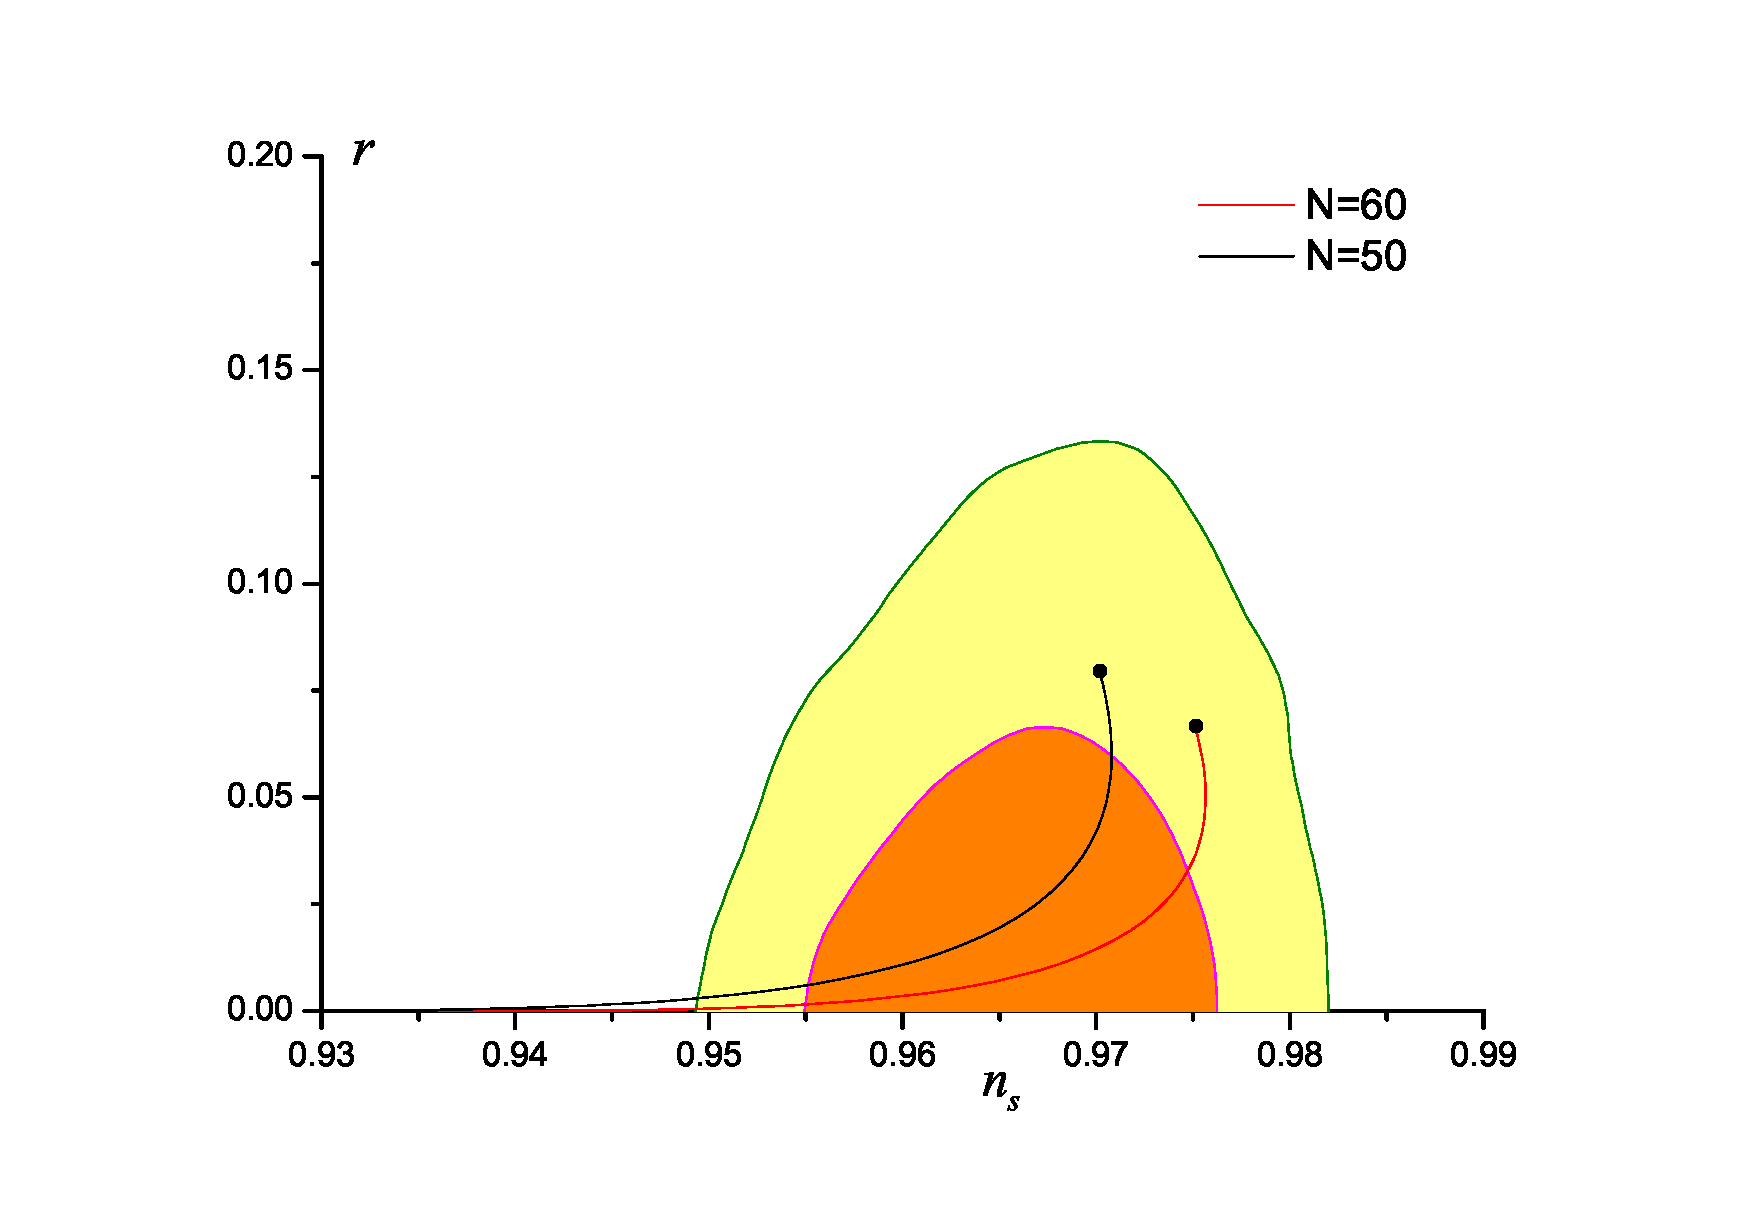
\includegraphics[width=5in]{Img/GN=50.eps}
  \caption{曲线为模型给出的$n_{s}-r$关系。其中参数$(n,
,p,q)$为$(2,1,2)$,黑色曲线和红色曲线分别对应e-folding数为$N=60$和$N=50$的数值结果。}\label{fig:GN-50}
\end{figure*}

图$(\ref{fig:Gn-1-2})$、$(\ref{fig:G2-p-4})$、$(\ref{fig:G2-1-q})$和$(\ref{fig:GN-50})$
展示了模型依据不同的$n$、$p$和$q$的值预言的$n_{s}-r$区域。等高线区域来自于
Planc 2015 年 TT+lowP
数据,基准尺度为$k_{\star}=0.002\text{Mpc}^{-1}$,$n_{s}-r$落在黄色和红色区域的可能性分别为$68\%$和$95\%$。

在图$(\ref{fig:Gn-1-2})$中,我们看到当$p=1$以及$q=2$时,随着$n$从$1$增加到$4$,曲线的位置越来越低,与
Planck
的数据越来越一致。图$(\ref{fig:G2-p-4})$中,选取参数$n=2$以及$q=4$,曲线从上到下
分别对应幂指数$p=3,2,1$。在图$(\ref{fig:G2-1-q})$中,选取参数$n=2$以及$p=1$,曲线从上到下分别对应幂指数$q=4,3,2$。可以看到三条曲线有一个汇聚点,该点正是$xi=0$的地方,也是最初势能为$V\propto
\varphi^{m
/n}$的暴胀模型给出的预言位置。图$(\ref{fig:GN-50})$中的两条曲线分别为$N=60$(黑线)和$N=50$(红线)的情况,从图中能够看出结果和
Planck 2015 的数据并不冲突。

最后,在暴胀结束后,标量场$\varphi$将会变得很小,直到$\varphi <
\sqrt{2}{\left(\kappa /n^2\right)}^{n
/(2n-2)}$后,动能项$(\ref{eq:kinetic-coefficient-of-Phi})$中的$\kappa$变得更加重要,于是标量场$\phi$取代$\varphi$成为动力学变量。这一阶段势能的形式变为${\left(\sum_m
\lambda_m \left\lvert
\phi\right\rvert^{m}\right)}^2$。随着场$\phi$继续减小,超对称破缺的质量项
$m_{\phi}\left\lvert\phi\right\rvert^2$开始主导势能的变化。
最终暴胀场将在原点附近来回振荡,通过与希格斯粒子耦合逐渐衰变为标准粒子来重新加热宇宙。这一重加热的过程和\citep{nakayama2010running}中描述的过程非常相似。

% 小结
\section{小结}

这一章首先介绍了在超引力框架内构造暴胀模型的历史。早期基于超引力的暴胀模型都会
遇到$\eta$问题,通常需要精细条件参数才能形成合理的暴胀过程。然而即便采用参数
调节的方式,在很多情况下也难以做到。后来通过引入平移对称性解决了这个问题。
接着回顾了跑动动能项暴胀模型。该模型的特点是在暴胀期间,拉氏量中动能项的变化
不能被忽略,从而标量场在暴胀过程中和暴胀结束后有不同的标量势。然后介绍了我们的
第一个工作,利用平移对称性以及带跑动动能项的多项式超势在超引力中构造了一个
单拐点暴胀模型。我们的模型预言了与Planck
2015的数据相一致的CMB功率谱,并且对标量谱指标$n_{s}$和张标比$r$的预测优于标量势
为$V\propto \varphi^{m
/n}$的原始模型。最后,在暴胀结束后,暴胀场在原点附近来回振荡,通过与希格斯粒子
的耦合逐渐衰变为标准粒子重新加热宇宙。

